\chapter{Bagging and Random Forests}

At a county fair, hundreds of people guess the weight of an ox. Most guesses are off by a lot, but in a famous
1906 contest, the \emph{median} of the guesses landed within 1\% of the true weight, closer than nearly every
individual guess. When many people make mistakes that are not the same mistakes, the mistakes cancel.

The last chapter ended with a weakness of decision trees: change the training data a little, and you may get a
very different tree. This chapter turns that weakness into a strength. Grow many different trees and let them
vote.

\section{The Wisdom of Crowds}
Suppose you have a panel of classifiers, each right 70\% of the time, and their mistakes are
\emph{independent}. Take a majority vote. The number of voters who are right follows a binomial distribution,
so the chance that the majority is right is a binomial tail probability:

\begin{center}
\begin{tabular}{c c}
\textbf{Number of voters} & \textbf{P(majority is right)} \\
\hline
1 & 0.700 \\
5 & 0.837 \\
25 & 0.983 \\
101 & 0.99999 \\
\end{tabular}
\end{center}

\begin{figure}[H]
\centering
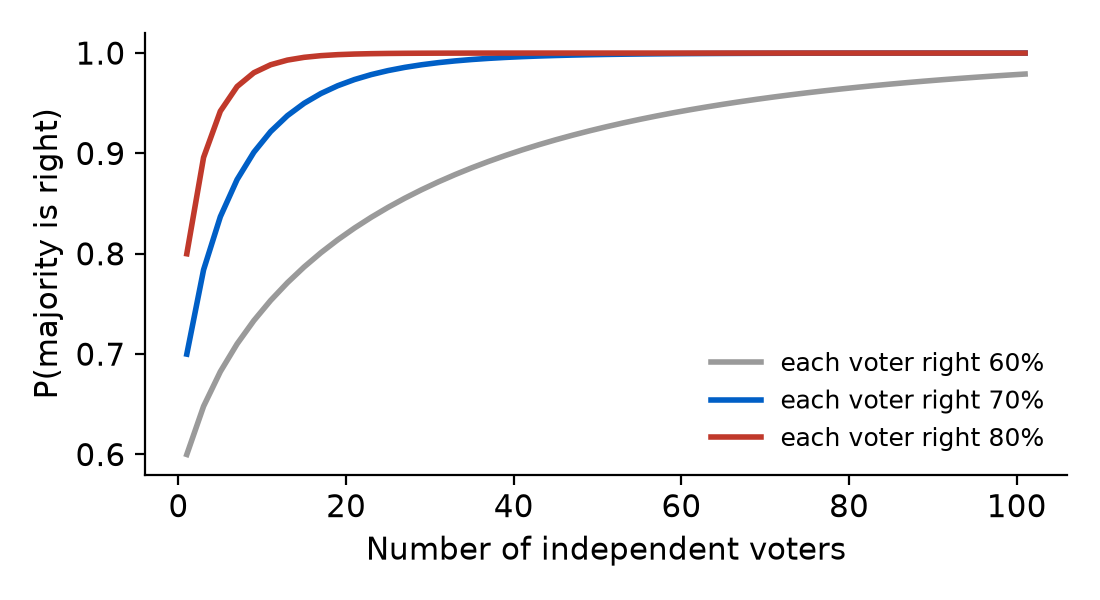
\includegraphics[width=0.6\textwidth]{crowd.png}
\caption{The chance that a majority of independent voters is right, for voters of three different
accuracies.}
\label{fig:crowd}
\end{figure}

The catch is the word ``independent.'' If all 101 voters are copies of the same classifier, they make the same
mistakes, and the vote is exactly as good as one of them. An ensemble helps only as much as its members
\emph{disagree}. The two methods in this chapter are ways to build trees that disagree.

\section{Bootstrap Aggregating}\index{bagging}
\newterm{Bagging}, short for bootstrap aggregating, trains each tree on a different \newterm{bootstrap
sample}\index{bootstrap sample}: $n$ points drawn from the original $n$ points \emph{with replacement}, the same
resampling you used for bootstrap intervals in the Simulation-Based Inference chapter. For classification, the
trees vote; for regression, their predictions are averaged.

\begin{figure}[H]
\centering
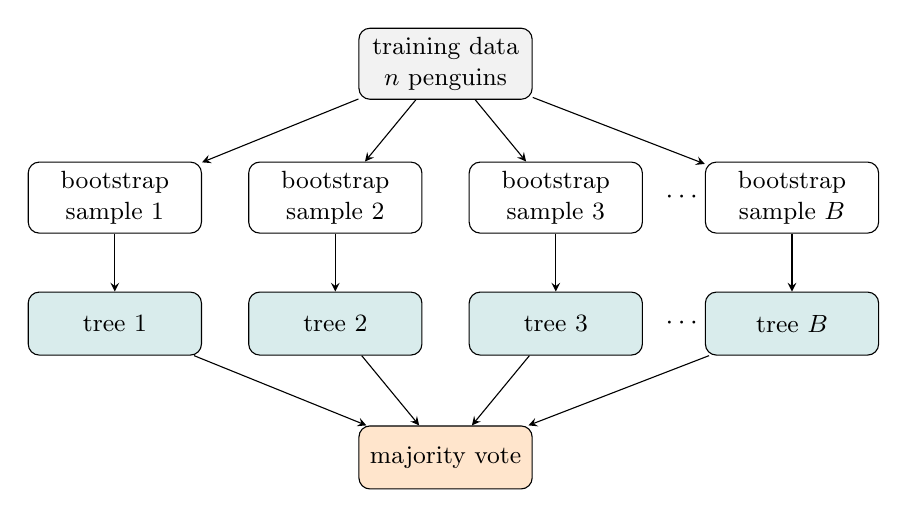
\begin{tikzpicture}[
  box/.style={draw, rounded corners, font=\small, align=center, minimum width=2.2cm, minimum height=0.8cm},
  >=stealth]
\node[box, fill=gray!10] (data) at (0,0) {training data\\$n$ penguins};
\foreach \i/\x in {1/-4.2, 2/-1.4, 3/1.4} {
  \node[box] (s\i) at (\x,-1.7) {bootstrap\\sample \i};
  \node[box, fill=teal!15] (t\i) at (\x,-3.3) {tree \i};
  \draw[->] (data) -- (s\i);
  \draw[->] (s\i) -- (t\i);
}
\node at (3.0,-1.7) {$\cdots$};
\node at (3.0,-3.3) {$\cdots$};
\node[box] (sB) at (4.4,-1.7) {bootstrap\\sample $B$};
\node[box, fill=teal!15] (tB) at (4.4,-3.3) {tree $B$};
\draw[->] (data) -- (sB);
\draw[->] (sB) -- (tB);
\node[box, fill=orange!20] (vote) at (0,-5) {majority vote};
\foreach \t in {t1, t2, t3, tB} \draw[->] (\t) -- (vote);
\end{tikzpicture}
\caption{Bagging: each tree learns from its own bootstrap sample, and the trees vote.}
\label{fig:bagging}
\end{figure}

\subsection{Why Bootstrap Samples Repeat}
Sampling with replacement means some points appear more than once and others not at all. A given point is missed
by one draw with probability $1 - \frac{1}{n}$, so it is missed by all $n$ draws with probability
$(1 - \frac{1}{n})^n$. For large $n$, this approaches $\frac{1}{e} \approx 0.368$. So each bootstrap sample
contains about $1 - \frac{1}{e} \approx 63.2\%$ of the distinct original points.

\textbf{Example}: For $n = 10$ points, a given point is missed by all 10 draws with probability
$(0.9)^{10} \approx 0.349$, so about 65\% of the distinct points appear in each bootstrap sample. For our 266
development penguins, the miss probability is $(1 - \frac{1}{266})^{266} \approx 0.367$, already very close to
$\frac{1}{e}$.

\section{Random Forests}\index{random forest}
Bagged trees still tend to look alike. If one feature is a very strong predictor, almost every tree puts it at
the top, and the trees make similar mistakes. A \newterm{random forest} adds one more source of randomness: each
time a tree chooses a split, it may consider only a random subset of $m$ features. Hiding the best feature from
some splits forces the trees to find other patterns, so they disagree more. A common choice is
$m = \sqrt{p}$ for classification, where $p$ is the number of features, and $m = p/3$ for regression.

Random forests, introduced by Leo Breiman in 2001, are one of the most reliable methods in machine learning:
they need little tuning, no scaling, and rarely overfit badly as you add trees.

\section{Out-of-Bag Error}\index{out-of-bag error}
About a third of the points are left out of each bootstrap sample. So each point can be predicted by the trees
that never saw it, about a third of the forest. The accuracy of these \newterm{out-of-bag} (OOB) predictions is
an honest estimate of how the forest does on new data, and it comes free with training. You can tune a random
forest without setting aside a separate validation set. (Keep the test set anyway, for the final report.)

\section{A Forest in Python}
The file \filename{trees.py} contains the tree code from the last chapter, with one change: \verb|grow| takes an
optional \verb|max_features|, and when it is set, each split looks at only that many randomly chosen features:
\begin{minted}{python}
    columns = range(X.shape[1])
    if max_features is not None:                 # random forest: a random subset
        columns = rng.choice(X.shape[1], size=max_features, replace=False)
    g, j, t = best_split(X, y, columns)
\end{minted}

Then \filename{forest.py} grows 200 trees for each method, keeping track of the test votes and the out-of-bag
votes as it goes:

\begin{minted}{python}
import numpy as np
from penguins import load_penguins
from trees import grow, predict

data = load_penguins()
names, y = np.unique(data["species"], return_inverse=True)
features = ["bill_length_mm", "bill_depth_mm", "flipper_length_mm", "body_mass_g"]
X = np.column_stack([data[f] for f in features])
order = np.random.default_rng(1).permutation(len(y))
dev, test = order[:266], order[266:]
X_dev, y_dev, n = X[dev], y[dev], len(dev)

def forest(n_trees, max_features, seed=0):
    rng = np.random.default_rng(seed)
    test_votes = np.zeros((len(test), 3))
    oob_votes = np.zeros((n, 3))
    single = []                                  # accuracy of each tree alone
    for b in range(1, n_trees + 1):
        sample = rng.integers(0, n, size=n)      # bootstrap: n draws with replacement
        tree = grow(X_dev[sample], y_dev[sample], max_features=max_features, rng=rng)
        guess = predict(tree, X[test])
        test_votes[np.arange(len(test)), guess] += 1
        single.append(np.mean(guess == y[test]))
        out = np.setdiff1d(np.arange(n), sample)   # penguins this tree never saw
        oob_votes[out, predict(tree, X_dev[out])] += 1
        if b in (1, 10, 50, 200):
            seen = oob_votes.sum(axis=1) > 0
            oob = np.mean(oob_votes[seen].argmax(axis=1) == y_dev[seen])
            acc = np.mean(test_votes.argmax(axis=1) == y[test])
            print(f"  {b:3d} trees: out-of-bag {oob:.3f}, test {acc:.3f}")
    print(f"  single trees on the test set: {min(single):.3f} to {max(single):.3f},"
          f" average {np.mean(single):.3f}")

print("Bagging (every split sees all 4 features)")
forest(200, max_features=None)
print("Random forest (every split sees 2 random features)")
forest(200, max_features=2)
\end{minted}

\begin{verbatim}
Bagging (every split sees all 4 features)
    1 trees: out-of-bag 0.918, test 0.955
   10 trees: out-of-bag 0.958, test 0.970
   50 trees: out-of-bag 0.970, test 0.955
  200 trees: out-of-bag 0.962, test 0.955
  single trees on the test set: 0.866 to 0.970, average 0.946
Random forest (every split sees 2 random features)
    1 trees: out-of-bag 0.918, test 0.955
   10 trees: out-of-bag 0.954, test 0.955
   50 trees: out-of-bag 0.974, test 0.970
  200 trees: out-of-bag 0.970, test 0.970
  single trees on the test set: 0.761 to 1.000, average 0.916
\end{verbatim}

The line \verb|test_votes[np.arange(len(test)), guess] += 1| adds one vote in row $i$, column \verb|guess[i]|, for
every test penguin $i$ at once. \verb|np.setdiff1d| finds the penguins that are not in the bootstrap sample.

\begin{center}
\begin{tabular}{l c c c}
\textbf{Method} & \textbf{Single trees (average)} & \textbf{OOB, 200 trees} & \textbf{Test, 200 trees} \\
\hline
one tree, all the data & --- & --- & 0.955 \\
bagging & 0.946 & 0.962 & 0.955 \\
random forest & 0.916 & 0.970 & 0.970 \\
\end{tabular}
\end{center}

Look at the single-tree column. Each random-forest tree is \emph{worse} on its own than a bagged tree (91.6\%
against 94.6\%), because it was sometimes denied the best feature. Their test accuracies range from 76\% to
100\%; they really do disagree. Yet the forest as a whole is the best of the three. That is the wisdom-of-crowds
effect: weaker but more independent voters make a stronger majority.

The differences here are small, because penguin species are easy to tell apart. (A single extra correct test
penguin is 1.5 percentage points.) On harder problems with many features, the gap between one tree and a forest
is usually much larger.

\begin{figure}[H]
\centering
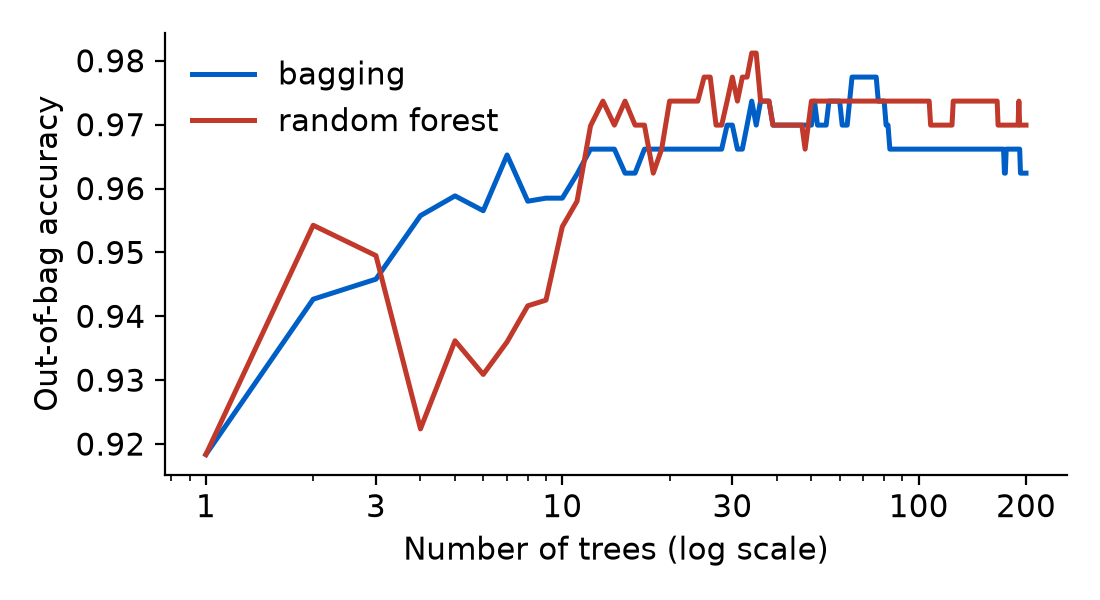
\includegraphics[width=0.62\textwidth]{oob_trees.png}
\caption{Out-of-bag accuracy as trees are added. It is noisy at first and then settles; adding more trees does
not cause overfitting.}
\label{fig:oob-trees}
\end{figure}

\section{What You Give Up}
A forest of 200 trees cannot be drawn on an index card. You lose the main attraction of a single tree, its
readability. Forests can still tell you which features matter most: add up how much each feature reduces the
impurity across all the splits in all the trees, a quantity called \newterm{feature importance}\index{feature
importance}. Forests are also slower: 200 trees take 200 times as long to train and to predict.

\begin{Exercise}[label=bag1, title=Probability a point is left out]
A data set has 5 points. What is the probability that a particular point is not chosen in any of the 5 draws of
a bootstrap sample?
\end{Exercise}
\begin{Answer}[ref=bag1]
$(1 - \frac{1}{5})^5 = (0.8)^5 \approx 0.328$.
\end{Answer}

\begin{Exercise}[label=bag2, title=Choosing m]
A classification problem has 16 features. How many features should each split consider in a random forest?
\end{Exercise}
\begin{Answer}[ref=bag2]
$m = \sqrt{16} = 4$.
\end{Answer}

\begin{Exercise}[label=bag3, title={Three voters}, space=3cm]
Three independent classifiers are each right with probability 0.8. What is the probability that their majority
vote is right?
\end{Exercise}
\begin{Answer}[ref=bag3]
The majority is right if all three are right or exactly two are:
$0.8^3 + 3(0.8^2)(0.2) = 0.512 + 0.384 = 0.896$.
\end{Answer}

\begin{Exercise}[label=bag4, title={Copies do not help}]
Explain why a forest of 100 trees grown on the \emph{same} data, with no bootstrap sampling and no random
features, would be no better than one tree.
\end{Exercise}
\begin{Answer}[ref=bag4]
Our tree-growing algorithm has no randomness, so every tree would be identical. All 100 would make exactly the
same predictions, the vote would always be unanimous, and the forest would be right exactly when the single tree
is.
\end{Answer}

\begin{Exercise}[label=bag5, title={Simulate a bootstrap}]
Use \verb|rng.integers(0, n, size=n)| to draw 1000 bootstrap samples of size $n = 266$. For each, compute the
fraction of distinct points with \verb|len(np.unique(sample)) / n|. What is the average? Compare with
$1 - (1 - \frac{1}{266})^{266}$.
\end{Exercise}
\begin{Answer}[ref=bag5]
\begin{minted}{python}
rng = np.random.default_rng(0)
n = 266
fractions = [len(np.unique(rng.integers(0, n, size=n))) / n for _ in range(1000)]
print(np.mean(fractions))
\end{minted}
The average is about 0.635, matching $1 - 0.367 = 0.633$ up to random variation.
\end{Answer}

\begin{Exercise}[label=bag6, title={One feature at a time}]
Run \filename{forest.py} with \verb|max_features=1|, so each split considers a single random feature. How do the
average single-tree accuracy and the forest's test accuracy change? Why?
\end{Exercise}
\begin{Answer}[ref=bag6]
The single trees get worse on average (89.3\%, ranging from 73\% to 100\%), because many splits are forced
to use a weak feature. The forest still gets 97.0\% of the test penguins right, with an out-of-bag accuracy of
97.4\%, because the votes of many varied trees cancel out much of that weakness. There is a trade-off: smaller $m$ makes the trees more independent but individually less
accurate.
\end{Answer}
